% \Image{Capa do livro (; )}{PNLD2022-001-01.png}
% \Image{Ilustração do livro (Acorde/Manuella Silveira; Acorde)}{PNLD2022-001-04.png}
% \Image{Ilustração do livro (Acorde/Manuella Silveira; Acorde)}{PNLD2022-001-05.png}
% \Image{Ilustração do livro (Acorde/Manuella Silveira; Acorde)}{PNLD2022-001-06.png}

\documentclass[11pt]{extarticle}
\usepackage{manualdoprofessor}
\usepackage{fichatecnica}
\usepackage{lipsum,media9}
\usepackage[justification=raggedright]{caption}
\usepackage[one]{bncc}
\usepackage[ayllon]{../edlab}
\usepackage{marginnote}
\usepackage{pdfpages}

\newcommand{\AutorLivro}{Luana Chnaiderman}
\newcommand{\TituloLivro}{O reino do meio da tarde}
\newcommand{\Tema}{Diversão e aventura}
\newcommand{\Genero}{Lendas; mitos; fábula}
%\newcommand{\imagemCapa}{./images/PNLD2022-001-01.jpeg}
\newcommand{\issnppub}{XXX-XX-XXXXX-XX-X}
\newcommand{\issnepub}{XXX-XX-XXXXX-XX-X}
% \newcommand{\fichacatalografica}{PNLD0001-00.png}
\newcommand{\colaborador}{Paulo Pompermaier}

\begin{document}

\title{\TituloLivro}
\author{\AutorLivro}
\def\authornotes{\colaborador}

\date{}
\maketitle

\tableofcontents


\begin{abstract}
Este material tem a intenção de contribuir para que você consiga desenvolver um trabalho aprofundado com a obra \textit{O reino do meio da tarde} em sala de aula.
Você encontrará informações sobre o autor, sobre o gênero e também 
algumas propostas de trabalho para a sala de aula que você poderá explorar livremente, 
da forma que considerar mais apropriada para os seus estudantes.

A junção da história poética de Luana Chnaiderman com as ilustrações delicadas e criativas de Andrés Sandoval faz de \textit{O reino do meio da tarde} um livro único. Isso porque a narrativa, só por sua poesia e sua premissa temporal, permite trabalhar diversas áreas e conhecimentos com os estudantes, partindo da interpretação artística da obra ao aprendizado de marcadores de tempo, como calendários e relógios, que são caros à narrativa.

Com as ilustrações, essas possibilidades ficam ainda mais amplas. Pois são desenhos de alta carga poética, com uma diversidade de cores, texturas, personagens e ambientes que fazem com que o trabalho interpretativo da imagem corra paralelo ao trabalho com o texto. 

Essa possibilidade de análise crítica das imagens é importante pois, cada vez mais, elas permeiam a sociedade em que vivemos. Como interpretamos 
imagens o tempo inteiro, não conseguimos perceber com clareza o quanto 
interpretá-las é uma atividade complexa. Ler imagens com competência, 
perceber seus recursos e nuances é parte importante do processo de apreensão, 
leitura e compreensão do mundo e de nossa existência. Antes de ler textos 
verbais, lemos textos visuais e os interpretamos a partir de nossas vivências, 
emoções e percepções.

Para além da narrativa, as ilustrações de \textit{O reino do meio da tarde} 
apresentam às crianças uma linguagem artística complexa.
As possibilidades são infinitas: explorar as cores, as formas, o posicionamento dos personagens na página e até mesmo a opinião e os sentimentos das crianças 
aprofundarão a leitura, aumentarão o repertório e incentivarão o desenvolvimento do vocabulário e da fluidez do discurso.


Ao longo do manual, todos esses aspectos serão explorados e relacionados a sugestões de atividades. Com isso, pretende-se oferecer ideias e inspirações para um trabalho que pode ser desenvolvido tanto a curto, quanto a médio e longo prazo. Sinta-se à vontade para personalizar a aula e torná-la sua, aplicando seus conhecimentos, sua 
personalidade e aproveite para fortalecer seu vínculo com a turma.
Boa aula!
\end{abstract}

\section{Sobre o livro}
Na curta e bela história de \textit{O reino do meio da tarde}, somos apresentados a uma fábula de intensa carga poética sobre um reino que vivia no meio da tarde, sem manhãs ou noites.

Sem noite, não era possível realizar atividades noturnas, como observar as estrelas ou ninar bebês; sem manhãs, os habitantes do reino não tinham vontade de dançar e não usufruíam o prazer de ver o sol nascer ou tirar um cochilo depois do almoço, quando o sol começa a se pôr e amainar.

Todos os dias nesse reino aquelas pessoas observavam o mesmo céu amarelo. Muitas partiram em busca do sol, para ver o dia nascer e morrer, como ferros de passar com asas e funis triunfantes, mas ninguém obteve sucesso. Os planetas não ouviam as preces e desejos daquele lugar sem horário.

Até que a Princesa Lua, desejosa de ver uma manhã e uma madrugada, saiu resoluta do seu reino. Iria pedir que sua terra tivesse manhã, tarde e noite, e tanto argumentou até que seu pedido foi atendido. Uma bela estrela do berçário das constelações foi colhida e levada para o Reino do meio da tarde.

A noite então invadiu o reino, e todos festejaram e celebraram em um baile iluminado por vagalumes e ritmado pelo som dos sapos, dançando até o dia raiar. Finalmente, assim, o reino pôde ser feliz, pois tinham o tempo: agora lá havia manhã, tarde e noite.

\reversemarginpar
\marginparwidth=5cm

%\marginnote{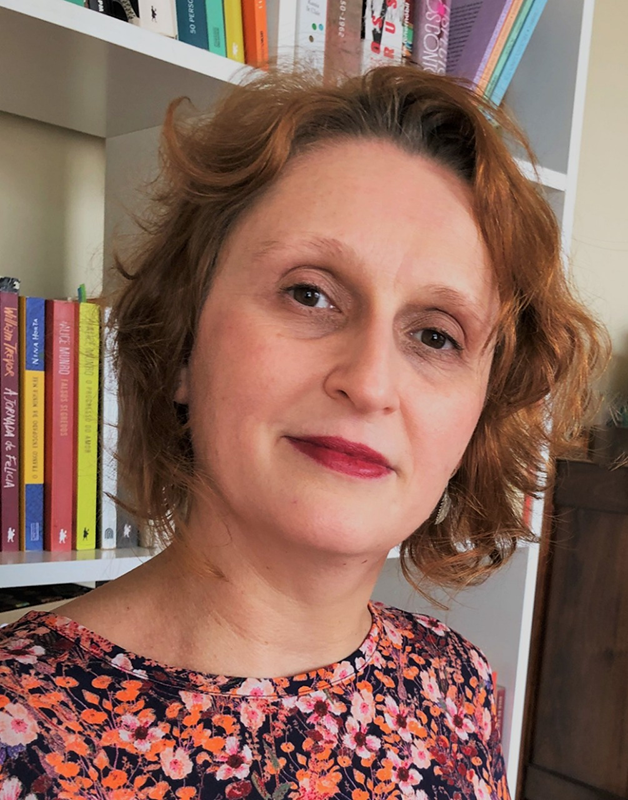
\includegraphics[width=\marginparwidth]{./images/PNLD2022-001-02.png}\\
%A autora Camila Werner (Arquivo pessoal)}


\section{Sobre os autores}

\paragraph{A autora} Luana Chnaiderman nasceu em São Paulo, onde se formou em Letras e também fez o mestrado na Universidade de São Paulo (\textsc{usp}). É professora de Português e dá cursos de escrita criativa. Publicou \textit{Minhocas}, (Cosac\&Naif, 2014) e \textit{Fuga} (\textsc{ftd}, 2017). Em 2019, seu livro \textit{Os animais domésticos e outras receitas} (Perspectiva, 2018), foi finalista do prêmio Jabuti em 2019.


\paragraph{O ilustrador} Andrés Sandoval, nascido em 1973 em São Paulo, é artista e ilustrador, formado em arquitetura e urbanismo pela Universidade de São Paulo (\textsc{usp}). A partir de 2003 começou a desenvolver projetos de livros, estampas e murais. Ilustrou e publicou livros por grandes selos editoriais brasileiros, como Companhia das Letras, Todavia e Editora Ubu. Participou da \textsc{x} e \textsc{xii} Bienal de Arquitetura de São Paulo, da exposição Cidade Gráfica no Itaú Cultural e Linhas de Histórias no \textsc{sesc} Santo André, Campinas e Araraquara. Entre seus parceiros de arquitetura e design, trabalha com Marcelo Rosenbaum, Grupo \textsc{sp}, \textsc{ps2} Design e Bloco Gráfico. Desenha as ilustrações das esquinas da revista \textit{Piauí}.


\Image{A lenda e o mito são narrativas fantasiosas transmitida pela tradição oral através dos tempos (The ponta cabeça; CC-BY-SA-4.0)}{PNLD2023-024-07.png}

\section{Sobre o gênero}

%55 caracteres
\paragraph{O gênero} O gênero deste livro é \textit{Lendas; mitos; fábula}. 

A lenda e o mito são narrativas fantasiosas transmitidas pela tradição oral através dos tempos. De caráter fantástico, as lendas e os mitos combinam fatos reais e históricos com eventos que não têm comprovação de acontecimento, a não ser pela palavra dos que sobraram para contar a história. As lendas e mitos de uma sociedade são fundamentais para que entendamos quem são essas pessoas e no que acreditam, bem como suas tradições. Uma lenda é verdadeira até que se prove o contrário. Com exemplos bem definidos em todos os países do mundo, as lendas e os mitos de um povo geralmente fornecem explicações plausíveis, e até certo ponto aceitáveis, para coisas que não têm explicações científicas comprovadas, como acontecimentos misteriosos ou sobrenaturais.

A fábula é uma narrativa curta em que os personagens principais geralmente são seres personificados. Esses seres apresentam características humanas, tais como a fala e traços de personalidade. Essas personagens podem ser também objetos animados ou deuses. Em cada história há uma lição de moral: uma mensagem de cunho educativo que busca conscientizar o leitor. A fábula tem estreita relação com o gênero conto, mas se diferencia pela centralidade dos personagens animais e pelo intuito de concluir a história com um ensinamento. É uma história que pode ser contada em prosa ou em versos. 

Sobre a origem da fábula, Douglas Tufano afirma que:

\begin{quote}
A fábula teria nascido provavelmente na Ásia Menor e daí teria passado pelas ilhas gregas, chegando ao continente helênico. Há registros sobre fábulas egípcias e hindus, mas sua criação é atribuída à Grécia, pois é onde a fábula passa a ser considerada como um tipo específico de criatividade dentro da teoria literária. 

Na Grécia, os primeiros exemplos de fábula datam do século \textsc{viii} a.C. Isso nos mostra, é claro, que Esopo não foi o inventor do gênero, mas sim o mais conhecido fabulista na Antiguidade como autor e narrador dessas pequenas histórias.\footnote{\textsc{tufano}, Douglas. \textit{Esopo: Fábulas completas}. São Paulo: Moderna, 2015.}
\end{quote}

Esopo foi um autor da Grécia Antiga a quem são atribuídas algumas das mais famosas fábulas, como \textit{A raposa e o cacho de uvas} e \textit{A galinha de ovos de ouro}. Diversas  histórias suas foram recontadas por La Fontaine, que é também um dos mais clássicos fabulistas do Ocidente.

No caso de \textit{O reino do meio da tarde}, há os elementos típicos das lendas e fábulas.
A história se inicia com o clássico ``era uma vez'', que já situa a narrativa no universo fantástico das lendas, estrutura típica das fábulas e histórias da carochinha. A descrição que se segue é de um reino mágico, caracterizado por uma condição especial (um lugar onde não havia tempo), seus habitantes fantásticos, que são os elementos do mundo personificados (ferros de passar alados, funis triunfantes, a princesa Lua etc.) e o comportamento particular de seus astros e planetas (sóis que habitam ninhos e estrelas ninadas em berçários de constelações).

A estrutura do enredo também segue o padrão das narrativas orais que caracteriza as lendas e fábulas: há uma situação inicial dada desde o início dos tempos (o reino bonito e tranquilo, escondido no meio das nuvens); o surgimento de um problema a ser contornado (os súditos que se cansaram de viver apenas na tarde e queriam o tempo em seu reino); as tentativas para solucionar o problema (as expedições dos cidadãos do reino em busca da manhã e da noite); o aparecimento do herói que contorna o problema (a princesa Lua que consegue trazer uma estrela ao reino e, assim, inaugurar a manhã e a noite); e o desfecho feliz, no qual o herói retorna a casa e o problema é solucionado (todos no reino ficam felizes, pois passaram a ter o tempo que tanto almejaram).

\section{Atividades}

\subsection{Pré-leitura}
\BNCC{EF01MA17}
\BNCC{EF01GE05}
\BNCC{EF01CI05}
\BNCC{EF02HI07}
\BNCC{EF03CI08}

\Image{O professor pode iniciar a atividade indagando os alunos sobre o tempo e as formas que eles conhecem de medi-lo. (CC-BY-SA-4.0)}{PNLD2023-036-03.jpg}

\paragraph{Tema} A passagem do tempo.

\paragraph{Conteúdo} Discussão em sala de aula sobre o tempo e suas diferentes marcações: percepções sensíveis da passagem do tempo, relógios, calendários e outros marcadores temporais.

\paragraph{Objetivo} O livro \textit{O reino do meio da tarde} parte da premissa de um reino que não tem tempo, logo vive apenas em um período do dia, a tarde. Para introduzir os estudantes na narrativa, propõe-se ao professor iniciar um debate sobre o tempo e as diferentes formas de marcá-lo. Assim, além de introduzir os estudantes no tema que será abordado na obra literária, o professor pode explorar e aprofundar a apreensão das crianças sobre competências importantes para seu período escolar, como a identificação de diferentes marcadores temporais. 

\paragraph{Justificativa} A partir do tema central do livro \textit{O reino do meio da tarde}, a passagem do tempo (e sua inexistência na história em questão), o professor tem a oportunidade de explorar com os alunos algumas competências fundamentais para o desenvolvimento humano e social. Em uma aula dialogada, o educador vai abordar os diferentes períodos do dia e sua divisão nos dias da semana, ensinando o uso do calendário e do relógio; apelar para as observações dos próprios estudantes sobre a passagem do tempo e os ritmos naturais; relacionar os períodos do tempo com seus astros, como o Sol, a Lua e as estrelas. Dessa forma, relaciona-se a atividade literária com o conhecimento de outras áreas, como a geografia e a ciência, e introduz-se o aluno em conhecimentos práticos e fundamentais do dia a dia, como observar o tempo e saber interpretar um calendário e um relógio.

\paragraph{Metodologia} O professor pode iniciar a atividade indagando os alunos sobre o tempo e as formas que eles conhecem de medi-lo. Em seguida, pode falar sobre as percepções sensíveis (tato, olfato, visão) que têm dos diferentes momentos do dia: do sol, do nascer do sol, do sol do meio-dia, do sol do fim da tarde, do início do anoitecer, da noite escura etc. Estimule-os a interagir e contar suas diferentes percepções dos momentos do dia, falando sobre seus momentos preferidos, o que chama mais atenção em cada período, como podemos perceber a passagem do tempo com outros órgãos que não os olhos. Por exemplo, falar sobre o calor que sentem na pele com o sol e o declínio gradual do calor e o acentuado frescor com o cair da noite.

Em seguida, o professor pode introduzir o uso dos principais marcadores de tempo da nossa sociedade. Os alunos sabem ler relógio de ponteiro? Se não, ensine-os a fazer a leitura, explicando a passagem dos números e sua relação com os momentos do dia. Fale sobre a orientação do sol do início ao final do dia e sua relação com os ponteiros e os números. É importante, igualmente, falar sobre a divisão no relógio de ponteiros do tempo em 12 horas, explicando essa convenção social e sua utilidade no dia a dia.

Quando o assunto se encaminhar para as horas que compõem o dia, o professor pode abordar o uso do calendário. Mostre como funciona o calendário, como os dias, semanas e meses estão dispostos. Fale sobre a sucessão de dias, semanas, meses e anos, sua relação com a passagem das horas (um dia de 24 horas uma semana de sete dias; um mês de quatro semanas; um ano de doze meses etc.).

Quando os alunos tiverem aprendido a ler e manusear o relógio e o calendário, o professor pode partir para uma atividade interpretativa. Pode fazer indagações como:

\begin{itemize}
\item Por que usamos o relógio?
\item E o calendário?
\item Qual a importância desses instrumentos para a vida cotidiana?
\item Qual relação vocês acham que esses instrumentos têm com a história que vamos ler nas próximas aulas?
\end{itemize}

Pode-se então distinguir os diferentes usos do tempo:

\begin{enumerate}
\item Culturais-tradicionais: festas populares, memória coletiva religiosa, memória familiar, etc.;
\item Usos mercantis do tempo: tempo para produção das coisas, controle do tempo para estudo e trabalho.
\end{enumerate}

Converse com o aluno sobre esses diferentes usos do tempo e como ambos coexistem nas sociedades contemporâneas. Como há o tempo em família, marcado por seus ritos e ritmos, o tempo das festas e feriados religiosos, e o tempo das fábricas, da escola, marcado pelo controle rigoroso do relógio.
Assim, pode-se introduzir --- e questionar --- a correlação entre tempo e remuneração, tempo e trabalho, além de refletir sobre a importância da disponibilidade de tempo.

\paragraph{Tempo estimado} Duas aulas de 50 minutos.

\Image{Quando os alunos tiverem aprendido a ler e manusear o relógio e o calendário, o professor pode partir para uma atividade interpretativa (CC-BY-SA-4.0)}{PNLD2023-036-04.png}

\subsection{Leitura}
\BNCC{EF15LP18}
\BNCC{EF15LP04}

\paragraph{Tema} Leitura dialogada do livro em sala de aula.

\paragraph{Conteúdo} Fazer uma leitura analítica que correlacione o texto e imagem, um dos elementos mais ricos deste livro.

\paragraph{Objetivo} A linguagem poética característica do livro \textit{O reino do meio da tarde} também se desdobra em suas ilustrações: predomina o tom lúdico e até surrealista das imagens, com figuras, cores e formas pouco usuais e de intensa carga poética. O objetivo da atividade é apreender essas diferentes dimensões do texto: a poesia do texto em relação com a poesia da imagem, levando o estudante a interagir e se indagar sobre as ilustrações que observa. 

\paragraph{Justificativa} Nos primeiros anos do ensino fundamental, é importante que o estudante aprenda a relacionar o texto escrito com as ilustrações ou outros recursos gráficos que acompanham a escrita. Trata-se de uma interação multissemiótica, na qual os aspectos gráfico-visuais do texto produzem efeitos de sentido. Saber identificar e analisar criticamente tais efeitos é competência incontornável para qualquer leitor. Ainda mais em nossa sociedade contemporânea, na qual as imagens são poderosas formas de comunicação, 
presentes desde outdoors e manuais de instrução até as inúmeras telas com que temos contato. Como interpretamos imagens o tempo inteiro, não conseguimos perceber com clareza o quanto interpretá-las é uma atividade complexa. Lê-las com competência, 
perceber seus recursos e nuances é parte importante do processo de apreensão, 
leitura e compreensão do mundo e de nossa existência. Antes de ler textos 
verbais, lemos textos visuais e os interpretamos a partir de nossas vivências, 
emoções e percepções.



\paragraph{Metodologia} O professor pode fazer uma primeira leitura com a classe, chamando a atenção para as imagens. Como o texto é bem curto, com palavras conhecidas e pouca dificuldade de apreensão da narrativa, a leitura propriamente é um processo rápido. Quando os alunos estiverem familiarizados com a história, o mais interessante é pedir que atentem-se em cada imagem e tentem relacioná-la com a história.

Pode-se pedir que descrevam, por exemplo, as cores e texturas das árvores; que observem as características dos moradores desse reino, como o cavaleiro sem cabeça do início e a silhueta de um homem que observa da torre; falar sobre a personificação dos objetos presentes nas imagens (os bules e chaleiras que ninam uma criança, os súditos exploradores que são ferramentas, o dia em formato de ninho-sol etc.).

Na imagem que acompanha o texto ``realizar caçadas noturnas / atrás de estrelas perdidas'', por exemplo, pode-se propor uma dinâmica de interpretação em que se pergunte aos alunos, estimulando a troca de impressões e interpretações entre eles:

\begin{itemize}
\item Qual é o elemento da imagem em que predomina a ideia de noite? (A cor preta);
\item A imagem contém apenas a ideia de noite? (Não, existem na ilustração partes iluminadas);
\item Qual parte da imagem alude às estrelas? (A parta clara, no canto superior esquerdo, que lembra o sol, que é também uma estrela)
\end{itemize}

E por aí vai, explorando elementos de cor, formas, personagens e texturas das imagens. Ao fim, pode-se concluir com uma brincadeira criativa, indagando-se os estudantes: por que as estrelas estariam perdidas? Apesar da poesia do texto, é uma questão que concerne à congruência e verossimilhança da narrativa: como é um reino sem tempo, em que nunca anoitece, não há estrelas, por isso elas estariam perdidas. Estimular esse tipo de interação é importante para desenvolver e aprimorar a observação crítica e uma boa interpretação que assimile tanto os elementos textuais quanto imagéticos da narrativa.

Cada imagem do livro, pelo seu alto teor poético e por suas diferentes dimensões, pode ser trabalhada da forma descrita acima.
Quando se fala, por exemplo, de ``ferros de passar alados'' e ``funis triunfantes'',
pode-se indagar os estudantes sobre o que eles pensam dessas imagens. Pedir que associem o ferro e o funil às suas respectivas representações gráficas, além de criar variações ao seu gosto, como pensar em outros objetos que poderiam ter característica animais ou humanas. A poesia aqui é menos sonora e mais imagética.

\paragraph{Tempo estimado} Duas aulas de 50 minutos.

\subsection{Pós-leitura}
\BNCC{EF02LP27}
\BNCC{EF15LP07}
\BNCC{EF02LP07}

\Image{Como diversos são os momentos do dia, bem com a influência dos astros no tempo da Terra, são muitas as possibilidades de trabalho. (CC-BY-SA-4.0)}{PNLD2023-036-05.jpg}


\paragraph{Tema} Criação literária.

\paragraph{Conteúdo} Produção escrita, ou desenho para os estudantes ainda não alfabetizados, que se inspire no mote do livro: os diferentes aspectos do tempo e uma vida imaginária sem tempo, que conheça apenas um dos momentos do dia.

\paragraph{Objetivo} Incentivar a expressão poética e textual dos estudantes. Acolher suas diferentes manifestações artísticas, estimulando o uso da imaginação e a assimilação da história de maneira pessoal e criativa.

\paragraph{Justificativa} A partir da apreensão poética do livro, passa-se ao momento de aplicar alguns conhecimentos trabalhados ao longo das aulas na produção de um pequeno texto, ou desenho, do próprio estudante. Assim, pode-se relacionar o universo artístico do livro, com sua premissa temporal e suas personagens fabulares, com a incipiente produção escrita de alunos que começam a aprender a escrever. Essa é uma forma de desenvolver o conhecimento gramatical e linguístico de forma afetiva e artística, pois relaciona os conhecimentos aprendidos sobre o livro com as regras gramaticais e as próprias experiências dos estudantes, que podem servir de base para a criação de sua pequenina história. Ademais, como se trata de um texto curto, partindo de alguns motes sugeridos pelo professor, o aluno pode pedir ajuda na composição para seus familiares, estimulando a interação em casa e a literacia familiar.

\paragraph{Metodologia} Já mais familiarizados com o livro, após ter interpretado a história e as diferentes imagens com o professor, os alunos devem passar à produção de um texto que parta do mote de escrita de \textit{O reino do meio da tarde}. Como diversos são os momentos do dia, bem com a influência dos astros no tempo da Terra, são muitas as possibilidades de trabalho:

\begin{itemize}
\item Criar um texto a respeito de um Reino que vivia no meio da noite;
\item Criar um texto a respeito de um Reino que vivia no comecinho da manhã;
\item Criar um texto a respeito de um Reino que tinha dois sóis ao mesmo tempo;
\item Criar um texto a respeito de um Reino em que a luz só vinha da Lua.
\item Criar um texto a respeito de um Reino no qual o Sol e a Lua apareciam no céu ao mesmo tempo.
\end{itemize}

O tema da redação não precisa ser fechado, respeitando a diversidade de narrativas que podem surgir a partir do mote temporal. Assim, é possível entrelaçar à história elementos biográficos, elementos do fantástico, ou mesmo da biografia de uma terceira pessoa pela qual o aluno nutre admiração. Além do mais, trata-se, em muitos casos, de um primeiro contato do aluno com o texto escrito, então ele não precisa elaborar muito. Basta um pequeno parágrafo, quase na forma de uma parlenda, em que ele pense no seu reino particular. Ele pode, por exemplo, escrever algo que viveu com sua família, ou alguma característica dela, em um reino do qual conseguiam enxergar todos os planetas do céu, ou no qual não existiam luzes artificiais, e todos ficavam no completo escuro após o por do sol.

As possibilidades e variações são infinitas. É importante que o professor estimule os alunos a partirem do tema proposto, um reino com uma característica temporal muito própria, mas que façam suas próprias criações, usando o tema temporal como uma inspiração de escrita. É possível, igualmente, relembrar determinadas passagens da história para inspirar os estudantes. Por exemplo, no \textit{Reino do meio da tarde}, seus habitantes conseguiram sair da tarde ao encontrar uma estrela. E como sairiam do reino do meio da manhã? Ou do reino da madrugada? Após a criação, estimule os alunos a conversar em sala e trocar suas experiências, dizendo quais características escolheram para seus reinos e compará-las com as dos colegas.

\paragraph{Tempo estimado} Duas aulas de 50 minutos.


\end{document}

